\documentclass[]{scrartcl}
\usepackage[utf8]{inputenc}
\usepackage{graphicx}
\usepackage{amsmath}
\usepackage{float}

\title{Technik und Technologie vernetzter Systeme  \\ Abgabe der Praktikumsaufgabe 1}

\author{Maria Lüdemann und Birger Kamp}

\begin{document}

\maketitle

\section{Projektschritt 1}
Nach der Durchführung des Projektschritts 1 anhand des Szenarios 1 haben wir einen Wireshark Mitschnitt gespeichert, der die Unterhaltung der Bestandteile des Netzwerks mitschneidet. Der Mitschnitt ist unten aufgeführt.

\begin{figure}[H]
	\centering
	\includegraphics[width=1\linewidth]{wireshark_1.png}
	\label{fig:wireshark_1}
\end{figure}

Hier zu sehen ist der Ablauf des Neighbor Solicitation Protokolls. Der Ablauf wird im folgenden Flussdiagramm noch einmal verdeutlicht. 


\begin{figure}[H]
	\centering
	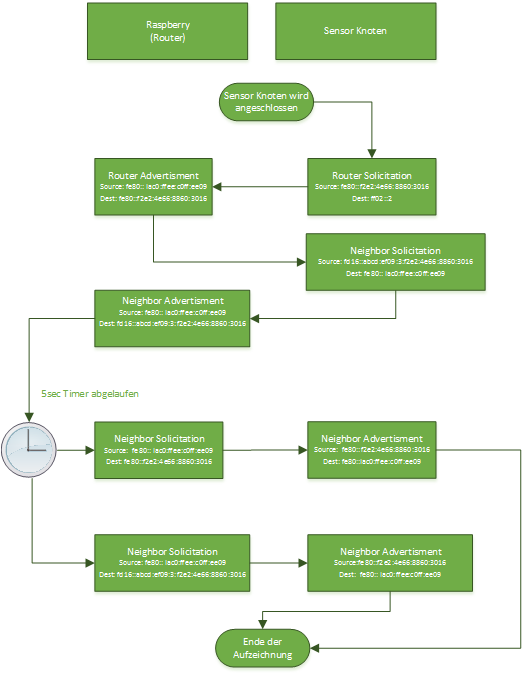
\includegraphics[width=1\linewidth]{flussdiagramm.png}
	\label{fig:flussdiagramm}
\end{figure}

Hier zu sehen ist, dass beim Anschließen des Sensor Knotens, selbiger nach dem Router fragt. Darauf antwortet der Raspberry Pi und gibt sich bekannt. Daraufhin erfragt der Sensor Knoten mit einer Neighbor Solicitation seine Nachbarschaft. Der Raspberry Pi antwortet mit einem Neighbor Advertisment. Auffällig ist dann aber, dass nach 5 Sekunden der Timer abläuft und die Nachbarschafts Anfragen erneut gesendet werden. Sowohl der Raspberry wie auch der Sensor Knoten senden Neighbour Solicitations und jeweilige Advertisements.\\

\textbf{Auffälligkeit}\\
Nach RFC 6775 (Abschnitt 3.3) sendet der Host einen NS an den Router mit einer gewissen Lifetime. Sollte die Lifetime ablaufen, dann erneuert der Host diesen Eintrag. Der Router fragt nicht aktiv nach beim Host. Die Anfragen nach dem Timeout sollten nach RFC 6775 nicht passieren!


\section{Projektschritt 2}
In Projektschritt 2 haben wir nach Szenario 2 unseren Versuchsaufbau ausgerichtet und durchgeführt. Im gemeinsamen Testlauf wurde durch Wireshark ein Mitschnitt der Kommunikation der Knoten erzeugt. Dieser lief über einige Zeit und umfasst insgesamt mehrere Tausend Nachrichten. In einem weiteren Schritt wurden alle Nachrichten die das RPL Protokoll betreffen analysiert um zu sehen wie es genutzt wird um eine Kommunikation aufzubauen. 

\subsection{Nachrichten und Informationsaustausch}
Die Nachrichten die im Rahmen des RPL Protokolls ausgetauscht werden sind entweder \textit{DODAG Information Object, DODAG Information Solicitation, Destination Advertisment Object oder Destination Advertisment Object Acknowledgment}. Dadurch werden die Informationen verteilt welche Knoten über wen zu erreichen sind. Wer Teil des Netzwekes ist und Verbindung zu wen anders hat. Mithilfe der Nachrichten kann ein Graph aufgebaut werden der es ermöglicht Nachrichten im Netz zu verteilen. 

Aufgrund der Nachrichten und deren Inhalt konnten wir in unserem Versuchsaufbau folgenden Baum entwerfen.
\begin{figure}[H]
	\centering
	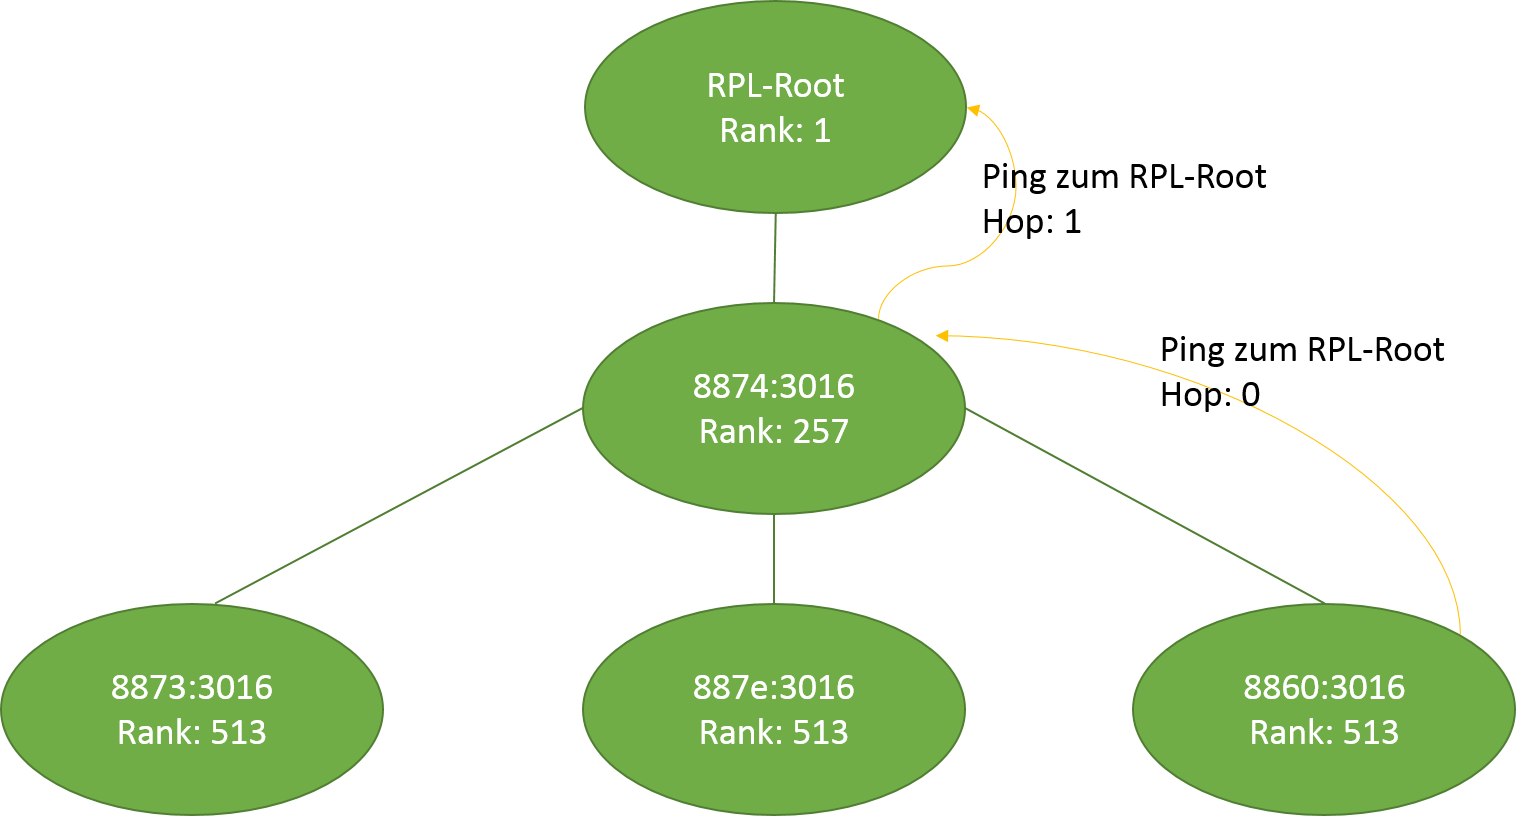
\includegraphics[width=1\linewidth]{RPL_Baum.png}
	\label{fig:RPL_Baum}
\end{figure}
\section{Projektschritt 3}

\end{document}